Earth observing satellites play an important role for many scientific and
meteorological applications. Their unique capability to provide frequent
observations of large parts of the globe allows meteorologists to predict the
weather and scientists to study the Earth and its atmosphere. Weather
predictions as well as the monitoring of the Earth's climate are of considerable
societal and economical value; a value that is likely to increase as the Earth's
climate warms.

The observations made by Earth observing satellite consist of measurements of
electromagnetic radiation, which is either reflected or emitted from the Earth
and its atmosphere. An example of such signals is given in
Fig.~\ref{fig:introduction:water_vapor}. The image shows infrared radiation
emitted from a low pressure system over the Mediterranean. The measured signal
in this example is the intensity of the radiation, represented from intense to
weak by the bright to dark coloring. At this specific frequency, the measured
radiation stems from water vapor and clouds in the atmosphere. Dry air, which
contains less water vapor, appears less opaque at the observing frequency. The
radiation emitted from dry air thus stems from lower down in the atmosphere
where temperatures are higher making the emitted radiation more intense. The
colors corresponding to intense radiation are thus indicative of dry air.
Moderate intensities correspond to moist air, while the lowest intensities stem
from high clouds that emit radiation at altitudes at which no significant
amounts of water vapor are present.

\begin{figure}[h!]
\centering
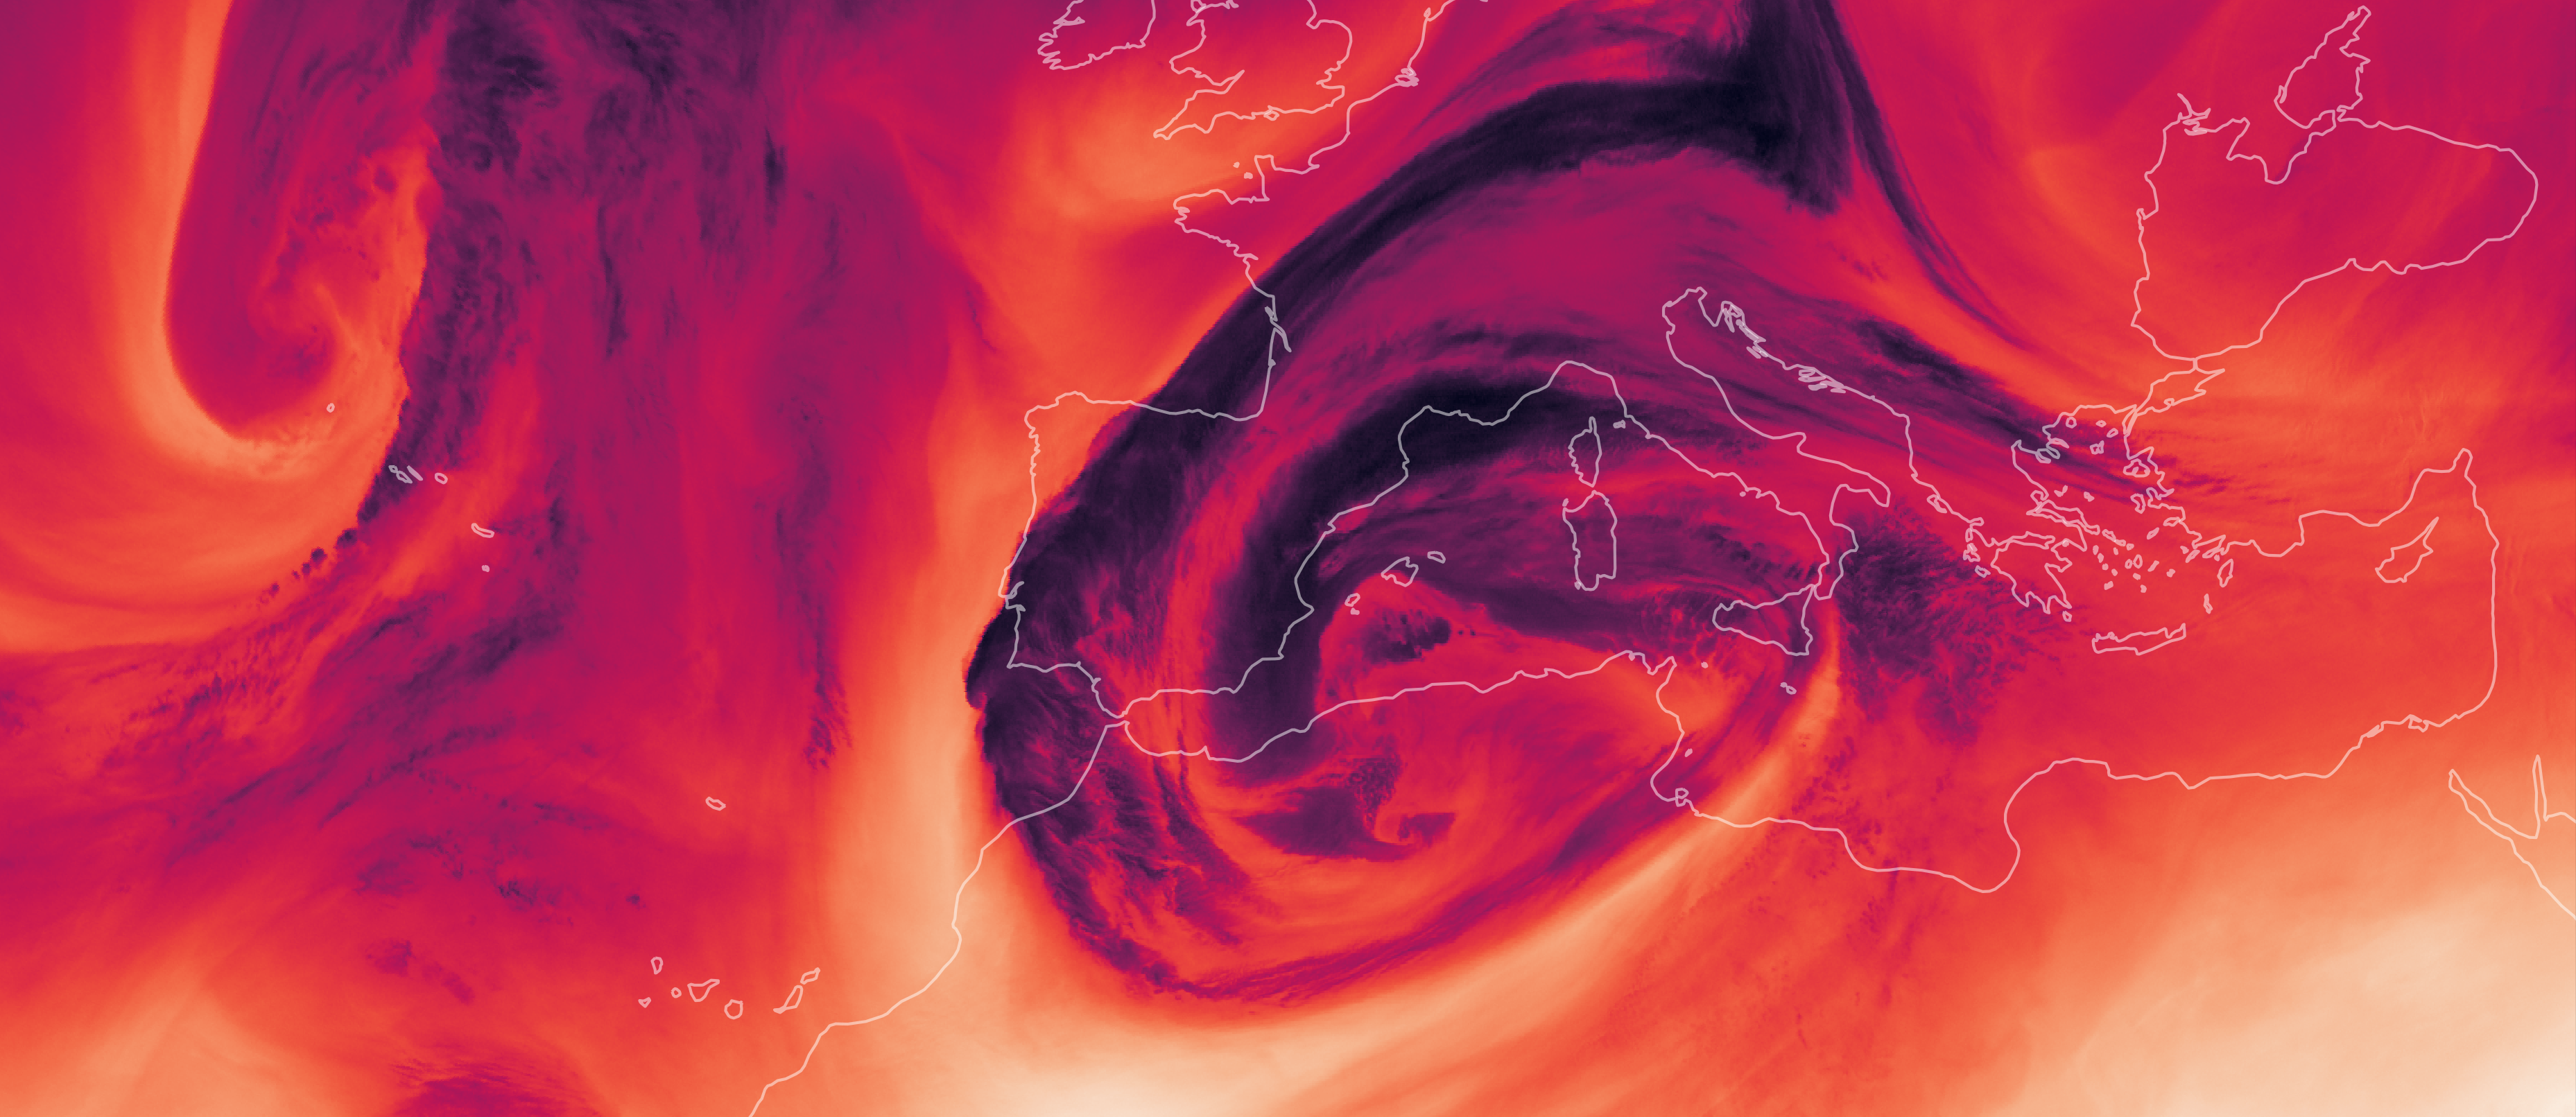
\includegraphics[width=\textwidth]{water_vapor}
\caption{Water vapor (white to red) and high clouds (purple to black) over the
Mediterranean as observed by the Spinning Enhanced Visible and Infrared
Imager at a wavelength of $\SI{6.2}{\micro \meter}$.}
\label{fig:introduction:water_vapor}
\end{figure}

As this example illustrates, knowledge of how the radiation observed by a
satellite is created allows an observer to infer moisture content and the
presence of high clouds from the satellite observations. Or, formulated more
generally: An atmospheric constituent that interacts sufficiently strongly with
this radiation, will create a signal that can be observed by the satellite. By
inverting the interaction of the atmosphere with the observed radiation, the
satellite observations can be used to estimate its properties. This
inversion, \textit{the retrieval}, relates satellite observations to physical
properties and thus informs the observer about the state of the atmosphere.

The subject of this thesis are computational methods to measure the properties
of clouds and precipitation using satellite observations. As will be explained
in more detail later on, these measurements are difficult, firstly, due to the
high variability in the appearance and composition of clouds and, secondly, due
to the complexity of their interaction with radiation. At the same time, such
measurements are highly relevant due to the important role that clouds and
precipitation play in the weather and climate system.

To set the scene for the discussion of satellite observations and retrieval
techniques in the subsequent chapters, this introduction aims to provide an
overview of the relevance of satellite observations of clouds and precipitation.
Beginning with the societal significance of water, the discussion will move on
to the scientific relevance observing water as it moves through the atmosphere.

\section{Water as resource}

Water is essential to life on Earth. It is the bloodstream of the biosphere
\citep{falkenmark04} and a fundamental resource to all forms of human
societies. It is common to categorize human water consumption into two types:
Blue water consumption refers to the consumption of fresh water taken from lakes,
rivers or ground water storage. The largest part of blue water consumption is
used to irrigate crops, while domestic and industrial use play minor roles. Blue
water consumption is distinguished from green water consumption, which refers to
the part of  precipitation over land that is released back to the atmosphere
through evaporation or transpiration. While often neglected, green water plays
an important role in providing water for rain-fed agriculture, which accounts
$60$ to $\SI{70}{\percent}$ of the global food production, and in sustaining
terrestrial ecosystems \citep{falkenmark04}.

Humans depend on water for food production both through irrigation from blue
water flows as well as the provision of soil moisture by green water flows.
Achieving food security has been recognized by the United Nations (UN) as a
sustainable development goal (SDG, \citeauthor{sdg}, \citeyear{sdg}). The large
contribution of food production to overall water consumption poses a challenge
to the management of water resources. Diverting more blue or green water flows
to the production of food reduces the amount of water that is available to
sustain terrestrial and aquatic ecosystems. There is thus potential for conflict
between the SDG to end hunger and the SDGs sustain terrestrial and aquatic
ecosystems \citep{falkenmark04}. Measurements of precipitation are a key
ingredient in the monitoring and modeling of water resources, which are required
to avoid and minimize conflicts between these competing functions of water.

An additional challenge for ensuring food security is the inter-annual
variability of water availability. It is particularly large in the arid and
semi-arid regions of the world \citep{falkenmark04}, where droughts are a
recurring feature of the climate. Also here satellite observations that allow
the monitoring of water resource are an important tool for the effective
management of droughts \citep{boyd13}.

%Water consumption is typically categorized into two classes: blue and
%green water consumption. Blue water consumption refers to 
%
%The consumption of water is typically categorized as blue water consumption,
%which refers to the extraction of surface water from rivers or ground water, and
%green water consumption, which refe to rain water consumed directly, for example
%to grow crops. Of the global blue water consumption, agricultural activity
%constitutes the largest part followed by industrial activity and domestic use
%\citep{falkenmark04}. Agriculture, however, also consumes large amounts of
%green water as $60$ to $\SI{70}{\percent}$ of the world's  food is produced on
%rainfed land.
%
%Water also plays an important role as source of energy. In the year 2020, energy
%produced from hydroelectric plants constituted one sixth of the global energy
%production \citep{eia21} and it can be expected that this portion will increase
%with the required decarbonization of the energy sector.


\section{The hydrological cycle}

Sustainable human water consumption is dependent on the replenishment of the
sources from which that water is obtained. Fresh water over land exists in the
form of glaciers, ice sheets, lakes and reservoirs, snow pack, wetlands and
rivers as well as a small part contained in the biomass. Water also exists
within the land surface in the form of soil moisture, permafrost and ground
water. The largest of the water that is available on the surface of the Earth is
stored in the oceans. Only a very small part is contained in the atmosphere - to
largest extent in the form of water vapor but also as clouds in the form of
liquid or frozen droplets \citep{abbott19}.

Despite containing only a tiny fraction of the global water reserves at any
given moment, the atmosphere is responsible for essentially all of the transport
of water from oceans to land, where it replenishes the water storages from which
it is available direct (blue) or indirect (green) consumption. The system of
fluxes between the different forms in which water exists on the surface of the
Earth is called  the hydrological cycle.

The illustration in
\ref{fig:introduction:water_cycle} provides an overview of the principal fluxes
of the hydrological cycle. The largest flux is that from the ocean to the
atmosphere. A large part of the water vapor that evaporates of the ocean never
reaches the land but instead returns to the ocean in form of precipitation. Only
about $\SI{10}{\percent}$ of the evaporation over oceans is transported to land,
where it may precipitate to replenish land-based freshwater reserves. A part of
that precipitation evaporates again allowing it to take part in the formation of
precipitation further inland.

On the scale of river basins, the inflow of water through the atmosphere is the
only sustainable source of fresh water \citep{falkenmark04}. Successful
monitoring of water resources is thus reliant upon the quantification of this
part of hydrological cycle. Since these fluxes occur across continental and
global scales, the currently only efficient way of measuring them is with the
help of satellite observations

\section{Weather and climate}

Water plays an important role in the weather system. When water evaporates, it
takes up energy from its environment. This energy, the latent heat, is released
when the air cools and the water vapor condensates. The release of latent heat
acts as fuel for the development of vigorous convective storms. The water that
is released by those storms in the form of precipitation can cause flooding and
land slides.

The ability to predict the weather has considerable value for society,
especially for high impact events involving extreme wind speeds or
precipitation. The availability of satellite observations has played an
important role in the steady improvement of weather forecast that took place
during the last three decades
\citep{bauer15}. Weather forecasting  systems use satellite data to
determine a best estimate of the current state of the atmosphere, which is then
evolved into the future to make a prediction. While most advanced forecasting
systems ingest satellite observations directly and are thus not dependent on
retrievals \citep{bauer10}, their use for improving model initialization for
short-range forecasts still being investigated
\citep{dehaan14, benjamin21}. Moreover, retrievals of precipitation and
cloud properties are l used by weather forecasters to gain situational awareness
and assess potential hazards such as flooding or mud slides.

%Despite the progress of the last decades, weather forecasts still struggle to
%produce accurate forecasts for specific meteorological contexts
%\citep{schafler18}. In many of those, the misrepresentation of the
%interaction of latent heat release through condensation and the large scale
%dynamics of the atmosphere were found \citep{rodwell13} to play a role.
%Improving the forecasts requires improving the representation of these processes
%in the model, which is where satellite-derived measurements of precipitation and
%clouds can help researchers better understand them.

Water is also an important actor in the climate system. Its primary effect is on
the Earth's energy budget. Water vapor is the most potent greenhouse gas and
thus contributes strongly to the retention of radiative energy emitted from the
Earth's surface. In the form of clouds, water both cools the Earth system
through the reflection of solar radiation and warms it through the absorption of
upwelling longwave radiation. Although the global effect of clouds is a
pronounced cooling, this effect varies regionally and with the properties of the
clouds.

Through its interactions with solar and IR radiation, water modulates
the incoming and outgoing energy fluxes of the atmosphere. In addition to that,
water plays an important role for energy fluxes within the climate system
through the uptake and release of latent heat. Transpiration and evaporation
account for a significant part of the heat released by the Earth's surface to
the troposphere, which shapes its thermodynamic structure. Latent heat also
plays an important role in the horizontal heat transport from the equator
to the poles \citep{stevens13}.

Instead a passive tracer of atmospheric dynamics the hydrological cycle must be
considered and activate component of the both the weather and climate system.
Scientists therefore rely on various observations of the hydrological cycle to
improve understanding of the climate system.


\section{A hotter planet}

The scientific evidence that the Earth system is heating up is
unambiguous \citep{ipcc21}. As the Earth system adapts to the increased
radiative forcing from greenhouse gases, its climate changes. These changes are
not uniform but vary across spatial scales and regions. To help societies adapt
to these changes, reliable regional predictions required. However, climate model
predictions at these scales remain tainted by uncertainties.

Together with the climate, also the hydrological cycle is changing: Increased
evaporation leads to more frequent droughts at the same time as total
precipitation in other regions is increasing. Extreme precipitation events are
strengthening and becoming more frequent. As for the climate, predicting changes
in the hydrological cycle is compounded by their regional and scale dependence.
At the scales of individual precipitation systems, precipitation increases
because of the higher capacity of warmer air to carry water vapor. However,
global evaporation is constrained to a smaller rate of change, which leads to a
coincident reduction of rain occurrence. These small scale changes are modulated
by changes in the general circulation, which defines the global distribution of
precipitation. Furthermore, these changes are masked by significant temporal
variability, which complicates their detection in observational data and
increases the uncertainty of short-term predictions.

Contributing to the difficulty of predicting the climate is that, as the climate
adapts to the radiative forcing caused by the increased greenhouse effect, the
resulting changes may act to increase or decrease the initial forcing.
These \textit{feedback mechanisms} determine the extent of the global warming
that will occur as a consequence of increased concentrations of carbon dioxide in the
atmosphere.

One of the important feedbacks is due to clouds. By reflecting incoming
short-wave radiation and the absorption of outgoing long-wave radiation, clouds
exert a strong influence on the Earth's energy budget. The net radiative
forcing by clouds is the sum of these two opposing effects. However their
strengths depends on the properties of the cloud such as their height
and composition as well as their location. Uncertainties in cloud
feedbacks remain the primary source of uncertainty in predictions of
the climate response to CO$_2$ emission.

Our understanding of climate change has progressed immensely during the last
decade but remains insufficient to make confident predictions at regional
scales. Such predictions are necessary for efficient climate change adaptation
and thus minimize human suffering. Given the complexity of the climate system,
advancing climate science is a multi-disciplinary challenge. Observations form
the basis of our understanding of the climate system. They are required to
improve and validate climate models as well as the identification of changes
in the climate system.


\section{Why satellites?}

Considering the importance of rain for a large range of human activities, it is
not surprising that humans have relied on observations in order to improve their
understanding of the weather system. The most direct and arguably intuitive way
to measure precipitation is through the use of \textit{rain gauges}. A rain
gauge consists of a cavity that captures rain and from which the accumulated
precipitation can be measured. First records of gauge measurements of rain date
back to as long as 400 years BC \citep{strangeways2000}. Today, dense gauge
measurements are available from all continents, however their density varies
from country to country and is oftentimes tied to the local population density.

The main disadvantage of rain gauges are the highly localized character of the
measurements, which limits their ability  to accurately capture the
spatial structure of precipitation on short time scales. Moreover, because
these measurements are performed by a large number of public and private
actors across the globe, not all of them are easily accessible for
scientists. Thus, only $\SI{1}{\percent}$ of the surface of the Earth is
estimated to be within a distance of $\SI{5}{\kiolo \meter}$ from the nearest
gauge measurement \citep{kidd17}.
by accessibility issues as well as their accessibility, which is hampered by

Over land, another important technique for measuring precipitation are
ground-based radars. These radars send out beams of radiation, which are
reflected by rain and snow. By measuring the amount of radiation that is
reflected back to the radar, precipitation within a radius several hundreds of
kilometers can be detected. Over land, ground-based radars play an important
role for real-time monitoring of precipitation. However, due to their high
installation and maintenance costs, their spatial availability is irregular and
typically tied to the local population density. In addition to that, the
availability and accuracy of radar measurements may by complex terrain as well
as the distance from the from the radar location, which limits the usefulness of
these observations for climatological purposes.

The relevance of clouds and precipitation for the hydrological cycle has been
known since before the times of Aristotle \citep{frisinger72}. Nonetheless, the
systematic study of clouds has long remained a secondary focus of modern
meteorology and it took until the 1970s until the importance of interactions
between clouds, weather and climate put them at the forefront of atmospheric and
climate research \citep{stephens02}. Traditionally, cloud observations were
conducted as parts of routine meteorological observations performed on land and
ships \citep{hughes84}. However, these observations were mostly qualitative in
nature indicating only the presence of clouds, a cloud class and their rough
height. 

The principal drawback of all of the measurement techniques discussed above is
their limited and irregular spatial coverage. This severely limits the
usefulness of the data for the monitoring of weather and climate. Observations
from satellites ideally complement surface based measurements as they can be
used to fill in the gaps between ground-based measurements.

